% ----------------------------------------------------
% Test results
% ----------------------------------------------------
\documentclass[class=report,11pt,crop=false]{standalone}
% Page geometry
\usepackage[a4paper,margin=20mm,top=25mm,bottom=25mm]{geometry}

% Font choice
\usepackage{lmodern}

\usepackage{lipsum}

% Use IEEE bibliography style
\bibliographystyle{IEEEtran}

% Line spacing
\usepackage{setspace}
\setstretch{1.20}

% Ensure UTF8 encoding
\usepackage[utf8]{inputenc}

% Language standard (not too important)
\usepackage[english]{babel}

% Skip a line in between paragraphs
\usepackage{parskip}

% For the creation of dummy text
\usepackage{blindtext}

% Math
\usepackage{amsmath}

% Header & Footer stuff
\usepackage{fancyhdr}
\pagestyle{fancy}
\fancyhead{}
\fancyhead[R]{\nouppercase{\rightmark}}
\fancyfoot{}
\fancyfoot[C]{\thepage}
\renewcommand{\headrulewidth}{0.0pt}
\renewcommand{\footrulewidth}{0.0pt}
\setlength{\headheight}{13.6pt}

% Epigraphs
\usepackage{epigraph}
\setlength\epigraphrule{0pt}
\setlength{\epigraphwidth}{0.65\textwidth}

% Colour
\usepackage{color}
\usepackage[usenames,dvipsnames]{xcolor}

% Hyperlinks & References
\usepackage{hyperref}
\definecolor{linkColour}{RGB}{77,71,179}
\hypersetup{
    colorlinks=true,
    linkcolor=linkColour,
    filecolor=linkColour,
    urlcolor=linkColour,
    citecolor=linkColour,
}
\urlstyle{same}

% Automatically correct front-side quotes
\usepackage[autostyle=false, style=ukenglish]{csquotes}
\MakeOuterQuote{"}

% Graphics
\usepackage{graphicx}
\graphicspath{{Images/}{../Images/}}
\usepackage{makecell}
\usepackage{transparent}

% SI units
\usepackage{siunitx}

% Microtype goodness
\usepackage{microtype}

% Listings
\usepackage[T1]{fontenc}
\usepackage{listings}
\usepackage[scaled=0.8]{DejaVuSansMono}

% Custom colours for listings
\definecolor{backgroundColour}{RGB}{250,250,250}
\definecolor{commentColour}{RGB}{73, 175, 102}
\definecolor{identifierColour}{RGB}{196, 19, 66}
\definecolor{stringColour}{RGB}{252, 156, 30}
\definecolor{keywordColour}{RGB}{50, 38, 224}
\definecolor{lineNumbersColour}{RGB}{127,127,127}
\lstset{
  language=Matlab,
  captionpos=b,
  aboveskip=15pt,belowskip=10pt,
  backgroundcolor=\color{backgroundColour},
  basicstyle=\ttfamily,%\footnotesize,        % the size of the fonts that are used for the code
  breakatwhitespace=false,         % sets if automatic breaks should only happen at whitespace
  breaklines=true,                 % sets automatic line breaking
  postbreak=\mbox{\textcolor{red}{$\hookrightarrow$}\space},
  commentstyle=\color{commentColour},    % comment style
  identifierstyle=\color{identifierColour},
  stringstyle=\color{stringColour},
   keywordstyle=\color{keywordColour},       % keyword style
  %escapeinside={\%*}{*)},          % if you want to add LaTeX within your code
  extendedchars=true,              % lets you use non-ASCII characters; for 8-bits encodings only, does not work with UTF-8
  frame=single,	                   % adds a frame around the code
  keepspaces=true,                 % keeps spaces in text, useful for keeping indentation of code (possibly needs columns=flexible)
  morekeywords={*,...},            % if you want to add more keywords to the set
  numbers=left,                    % where to put the line-numbers; possible values are (none, left, right)
  numbersep=5pt,                   % how far the line-numbers are from the code
  numberstyle=\tiny\color{lineNumbersColour}, % the style that is used for the line-numbers
  rulecolor=\color{black},         % if not set, the frame-color may be changed on line-breaks within not-black text (e.g. comments (green here))
  showspaces=false,                % show spaces everywhere adding particular underscores; it overrides 'showstringspaces'
  showstringspaces=false,          % underline spaces within strings only
  showtabs=false,                  % show tabs within strings adding particular underscores
  stepnumber=1,                    % the step between two line-numbers. If it's 1, each line will be numbered
  tabsize=2,	                   % sets default tabsize to 2 spaces
  %title=\lstname                   % show the filename of files included with \lstinputlisting; also try caption instead of title
}

% Caption stuff
\usepackage[hypcap=true, justification=centering]{caption}
\usepackage{subcaption}

% Glossary package
% \usepackage[acronym]{glossaries}
\usepackage{glossaries-extra}
\setabbreviationstyle[acronym]{long-short}

% For Proofs & Theorems
\usepackage{amsthm}

% Maths symbols
\usepackage{amssymb}
\usepackage{mathrsfs}
\usepackage{mathtools}

% For algorithms
\usepackage[]{algorithm2e}

% Spacing stuff
\setlength{\abovecaptionskip}{5pt plus 3pt minus 2pt}
\setlength{\belowcaptionskip}{5pt plus 3pt minus 2pt}
\setlength{\textfloatsep}{10pt plus 3pt minus 2pt}
\setlength{\intextsep}{15pt plus 3pt minus 2pt}

% For aligning footnotes at bottom of page, instead of hugging text
\usepackage[bottom]{footmisc}

% Add LoF, Bib, etc. to ToC
\usepackage[nottoc]{tocbibind}

% SI
\usepackage{siunitx}

% For removing some whitespace in Chapter headings etc
\usepackage{etoolbox}
\makeatletter
\patchcmd{\@makechapterhead}{\vspace*{50\p@}}{\vspace*{-10pt}}{}{}%
\patchcmd{\@makeschapterhead}{\vspace*{50\p@}}{\vspace*{-10pt}}{}{}%
\makeatother
\makenoidxglossaries

\newacronym{radar}{RADAR}{Radio Detection and Ranging}
\begin{document}
\ifstandalone
\tableofcontents
\fi
% % ----------------------------------------------------
\section{Testing and results \label{ch:T_R}}
% ----------------------------------------------------




\subsection{Is the model performance better if MFCCs are used as input features?}


\subsection{Comparing depth of neural networks}

As discussed in section \ref{ch:Feature_Extraction}, A set of spectrograms were generated when each windowing method was applied to the datasets. In total there were three sets of spectrograms. Each set of spectrograms was passed through a shallow and deeper CNN, with the data shown in figure \ref{fig:SpecCNN}.

\begin{figure}[hbt!]
    \begin{subfigure}[b]{0.5\textwidth}
        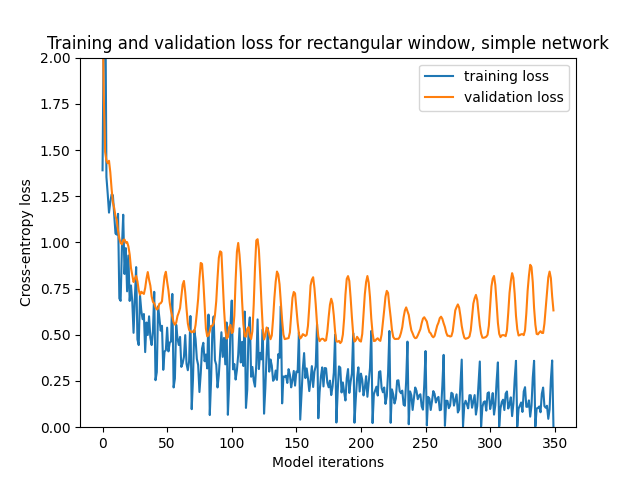
\includegraphics[width=\linewidth]{Images/rectangularSimple.png}
        \caption{Rectangular filter applied to data passed through a shallow CNN}
        \label{fig:RectShallow}
    \end{subfigure}
    \hfill
    \begin{subfigure}[b]{0.5\textwidth}
        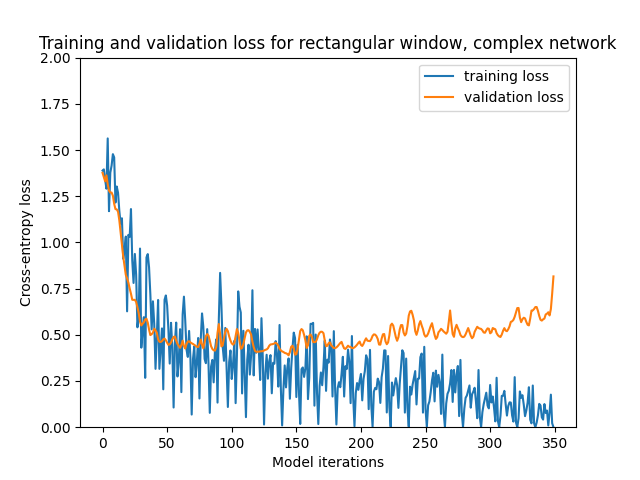
\includegraphics[width=\linewidth]{Images/rectangularComplex.png}
        \caption{Rectangular filter applied to data passed through a deeper CNN}
        \label{fig:RectDeeper}
    \end{subfigure}
    \hfill
    \begin{subfigure}[b]{0.5\textwidth}
        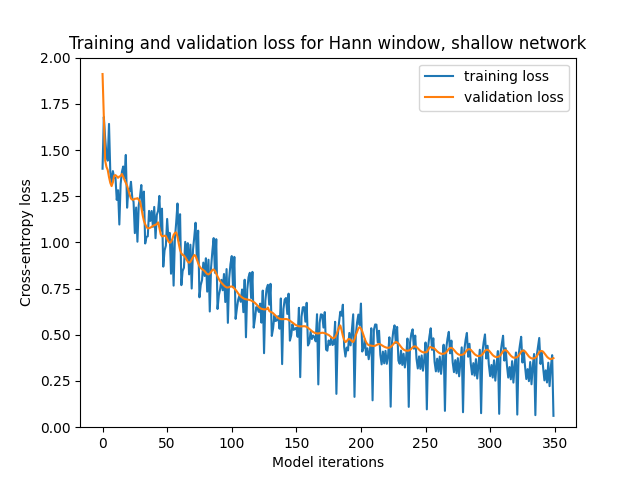
\includegraphics[width=\linewidth]{Images/hannSimple.png}
        \caption{Hann filter applied to data passed through a shallow CNN}
        \label{fig:HannShallow}
    \end{subfigure}
    \hfill
    \begin{subfigure}[b]{0.5\textwidth}
        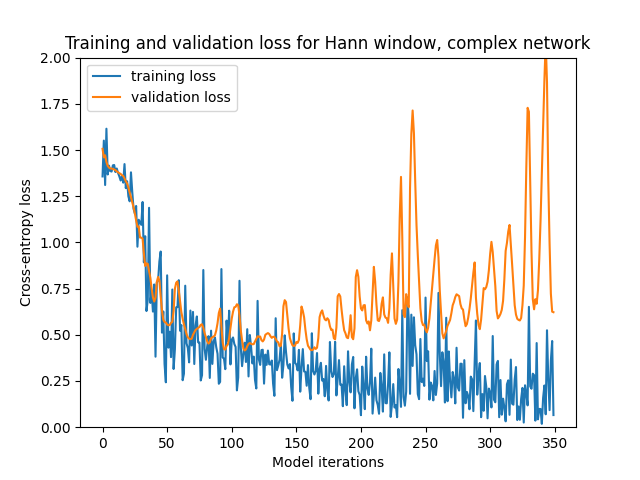
\includegraphics[width=\linewidth]{Images/hannComplex.png}
        \caption{Hann filter applied to data passed through a deeper CNN}
        \label{fig:HannDeeper}
    \end{subfigure}
    \hfill
    \begin{subfigure}[b]{0.5\textwidth}
        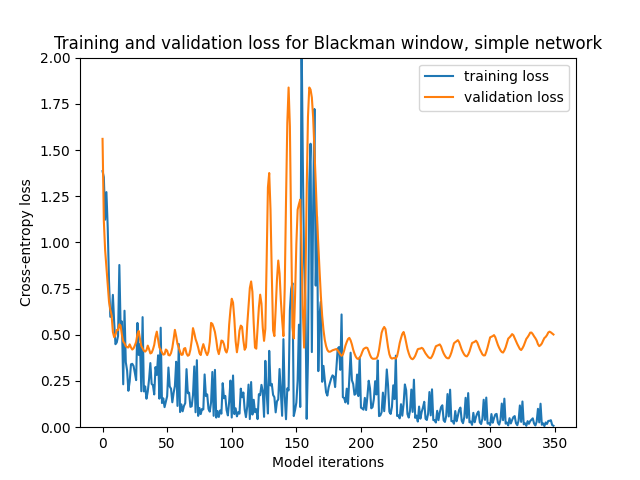
\includegraphics[width=\linewidth]{Images/blackmanSimple.png}
        \caption{Blackman filter applied to data passed through a shallow CNN}
        \label{fig:BlackmanShallow}
    \end{subfigure}
    \hfill
    \begin{subfigure}[b]{0.5\textwidth}
        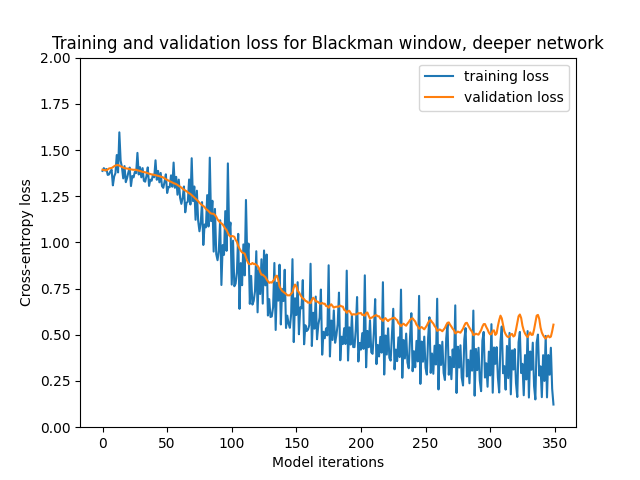
\includegraphics[width=\linewidth]{Images/blackmanComplex.png}
        \caption{Blackman filter applied to data passed through a deeper CNN}
        \label{fig:BlackmanDeeper}
    \end{subfigure}
    \caption{Result after Spectrograms were passed through neural networks of variable depth}
    \label{fig:SpecCNN}
\end{figure}

The graphs show the training and validation losses as the number of model iterations increase. Each model was trainged for 25 epochs (amounting to just over 350 iterations with batch sizes of 16). Models were trained at a learning rate of 0.0002, after experimentation revealed that gave relatively stable results. Models were trained on a single random split of the training data into 80\% training data and 20\% validation data.

The clear result from all three windowing methods is that the more complex model tends to overfit to the data more heavily within the number of iterations trained. Deeper networks have increased complexity and more features, making it possible for them to fit more finely to the training data; however, this can have the side effect of overfitting on the training data and poor validation performance. Deeper neural networks are also more likely to experience problems relating to vanishing and exploding gradient. This tends to happens to gradients when they are passed through multiple layers of learning during the training process, slowing it down.

The best-case validation performance for the `shallow' network is better than that of the `deeper' network for both the rectangular and Blackman windows, and is comparable for the Hann window. Training a deeper neural network in general should take longer to train due to more parameters having to be learnt, since the deeper networks have more layers where the learning process involves an interative process of adjusting the the learning parameters in an attempt to improve model accuracy, as well as increased complexity. Overall, the added computational requirements of the `deeper' network cannot be justified.

A limitation of this comparison came from the splitting of data; the single training-validation split could yield results that are overly dependent on the specific split of data. Across the three window types, the conclusion that the simple model is more useful can still be deemed valid, but a meaningful evaluation of the difference between the window types cannot be made from this data.



\subsection{Comparing windowing types}







Bearing in mind that the rectangle and Blackman window have the worst and best attenuation of spectral leakage respectively, Table \ref{tab:Mean_Acc} shows that degree of spectral leakage attenuation affects the performance of shallower CNNs. The CNN model that is trained on the data that was processed with the rectangular window had poorer performance in comparison to the same data processed with Blackman and Hann windows. This shows a direct link between spectral leakage and the model accuracy. The models trained with data that was processed with the Blackman and Hann windows performed with the same accuracy. This was expected since both windows are great in limiting spectral leakage, and reducing the variability of the model. 





Shallow CNNs, which are far more computationally efficient and require fewer iterations to become perfectly fit, still has room for improvement, specifically when it comes to the performance of the model on unseen data. This is why k-fold cross-validation is used. 

K-fold cross-validation is a is very powerful when it comes to assessing the model's performance on unseen data. The dataset is divided into 'k' subsets referred to as folds. The model is trained 'k' times and uses 'k-1' folds for training and '1' fold for validation. This would provide a more comprehensive result on the model performance. 

By applying this to the shallow CNN trained with the data processed with various windowing methods, it provides a guide as to which model parameters to tune. 

Figure \ref{fig:K-Fold} shows the mean, min and standard deviation of the k-fold window type analysis. Table \ref{tab:k-fold-average} then gives the accuracy of the last 5 k-fold iterations. 

\begin{figure}[hbt!]
    \begin{subfigure}[b]{0.5\textwidth}
        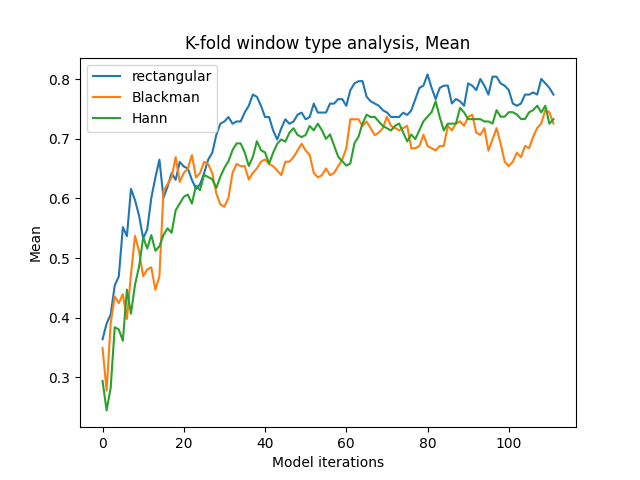
\includegraphics[width=\linewidth]{Images/kfoldMean.png}
        \caption{Mean k-fold validation results}
        \label{fig:KMean}
    \end{subfigure}
    \hfill
    \begin{subfigure}[b]{0.5\textwidth}
        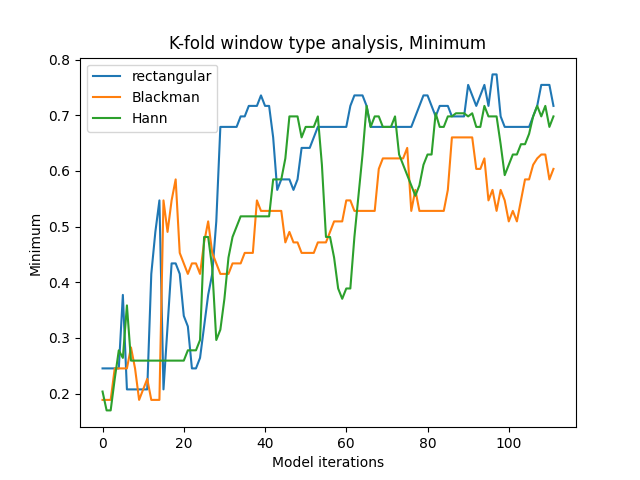
\includegraphics[width=\linewidth]{Images/kfoldMinimum.png}
        \caption{Minimum k-fold validation results}
        \label{fig:KMin}
    \end{subfigure}
    \hfill
    \begin{subfigure}[b]{0.5\textwidth}
        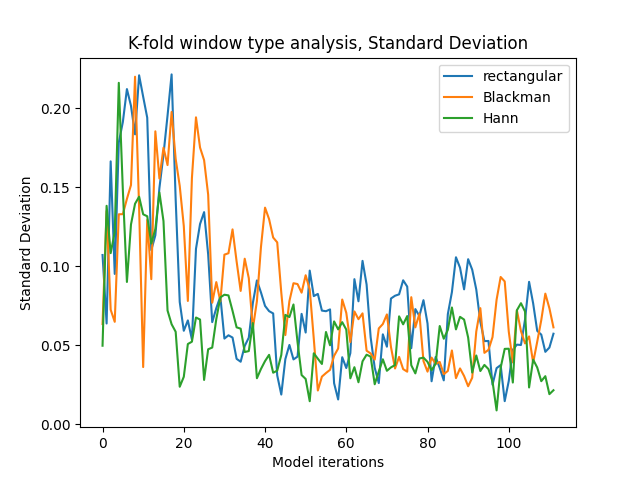
\includegraphics[width=\linewidth]{Images/kfoldStandard Deviation.png}
        \caption{Standard deviation k-fold results}
        \label{fig:KStd}
    \end{subfigure}
    \caption{Graphical Representation of K-Fold Cross Validation Results}
    \label{fig:K-Fold}
\end{figure}
 
\begin{table}[h]
\centering
\begin{tabular}{|l|l|}
\hline
\textbf{Window} & \textbf{k-fold accuracies (\%)} \\
\hline
Rectangle & [78.9 83.8 83.77.2 76.4 72.3] \\
Blackman & [63.1 77.2 64.0 82.6 67.4] \\
Hann & [69.3 78.7 70.9 73.9 77.9] \\
\hline
\end{tabular}
\caption{k-fold validation data for the last 5 k-fold iterations}
\label{tab:k-fold-average}
\end{table}

Figures \ref{fig:KMean} and \ref{fig:KMin} shows that the model trained with data processed with the rectangular window had the highest average accuracy in comparison to the data processed with the Blackman and Hann windows. Although, the data processed with the Hann window was not far off comparison. The model trained with data processed with the Blackman window did not perform as well as it was expected to. This shows that the higher frequency resolution associated with rectangular windows had an effect on the performance of shallow CNNs. The features extracted could likely be less affected by spectral leakage. 

Figure \ref{fig:KStd} told a completely different story. Even though the model trained with data processed with the rectangular window had the best overall accuracy, the variability was the the highest, looking at the region of model iterations between 50 and 100. The other models had less variability. 

% ----------------------------------------------------
\ifstandalone
\bibliography{../Bibliography/References.bib}
\printnoidxglossary[type=\acronymtype,nonumberlist]
\fi
\end{document}
% ----------------------------------------------------